\documentclass[adraft,creativecommons]{eptcs}
\usepackage[utf8]{inputenc}

\usepackage{underscore}

\usepackage[T1]{fontenc}
\usepackage{mathpartir}
\usepackage{amssymb}
\usepackage{amsmath}
\usepackage{braket}
\usepackage{xspace}
\usepackage[capitalize]{cleveref}
\crefformat{section}{\S#2#1#3}
% \crefformat{figure}{Fig. #2#1#3}

% \usepackage{adjustbox}
\usepackage{tikz}
\usetikzlibrary{quantikz}

% From: https://tomhennigan.blogspot.com/2012/01/grouped-emails-in-latex-with-href-and.html
\newcommand{\mailtodomain}[1]{\href{mailto:#1}{\nolinkurl{#1}}}

\usepackage{xcolor}
\definecolor{dkgreen}{rgb}{0,0.35,0}

\usepackage{listings}
\lstloadlanguages{Haskell}
\lstdefinelanguage{QHaskell}{
    language     = Haskell,
    morekeywords = {bool, qbit, U, C, meas, apply, to},
}

\lstset{
    basicstyle=\small\ttfamily,
    frame=single,
    captionpos=b,
    numbers=left,
    numberstyle=\tiny\color{gray},
    flexiblecolumns=false,
    basewidth={0.5em,0.5em},
    commentstyle=\color{dkgreen},
    keywordstyle=\bfseries\color{blue},
    stringstyle=\color{violet},
    literate=
        {√}{{$\surd$}}1
        {⇐}{{$\Leftarrow$}}1 {⇒}{{$\Rightarrow$}}2
        {->}{{$\rightarrow$}}2
        {|}{{$\vert$}}1 {⟩}{{$\rangle$}}1
        {∧}{{$\wedge$}}1 {∨}{{$\vee$}}1
        {∈}{{$\in$}}1 {Π}{{$\Pi$}}2
        {∃}{{$\exists$}}2 {∀}{{$\forall$}}2
        {⊗}{{$\otimes$}}1 {⊕}{{$\oplus$}}1
        {⊤}{{$\top$}}2
        {=q}{{$=_q$}}2 {=c}{{$=_c$}}2
        {α}{{$\alpha$}}1 {β}{{$\beta$}}1
        {ψ}{{$\psi$}}1
        {_i}{{$_i$}}1 {_x}{{$_x$}}1 {_y}{{$_y$}}1
        {\ .\ }{{$\cdot$}}1
        {β00}{{$\beta_{00}$}}2
}

\usepackage{blindtext}

\def\titlerunning{Quantum Hoare Type Theory}
\def\authorrunning{Kartik Singhal}

\title{\titlerunning}

\author{
\authorrunning
\institute{University of Chicago}
\email{\mailtodomain{ks@cs.uchicago.edu}}
}

\begin{document}

\maketitle

\begin{abstract}
    \blindtext
\end{abstract}

\thispagestyle{empty}

\tableofcontents

\listoffigures

\lstlistoflistings

% \listoftables

\clearpage

\pagenumbering{arabic}

\section{Introduction}

\blindtext

\section{Background}

TODO:

- Hoare logic and Hoare Type Theory

- basics of quantum computing (4 laws, superposition and entanglement, pure vs mixed states)

- Quantum Hoare Logic

- define the meaning of subspace/projector-based predicates/propositions.

\section{Quantum Hoare Type Theory}

TODO:

- define the syntax of the language

- proof rules at each step

\subsection{Examples}

\blindtext

\subsubsection{Bell states}

Our simplest example involves creation of a Bell (or EPR) state which is one of the four maximally entangled quantum states of two qubits. Specifically, we will create a circuit (\cref{fig:bell00}) to produce the first Bell state which we will write in the mnemonic notation as $\ket{\beta_{00}} = (\ket{00}+\ket{11})/\sqrt{2}$.

\begin{figure}
    \centering
    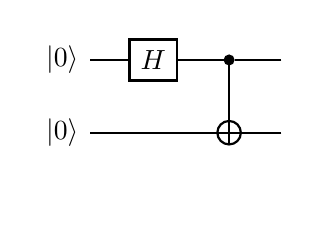
\begin{tikzpicture}
        \node[scale=1.0] {
            \begin{quantikz}
                \lstick{$\ket{0}$} & \gate{H} & \ctrl{1} & \qw \\
                \lstick{$\ket{0}$} & \qw      & \targ{}  & \qw \\
            \end{quantikz}
        };
    \end{tikzpicture}
    \caption{Circuit to prepare the first Bell state}
    \label{fig:bell00}
\end{figure}

\lstinputlisting[language=QHaskell,lastline=7,caption=Generating Bell state]{bell00.qh}

This circuit corresponds to a suspended quantum computation that can be composed with other circuits. It takes no input and returns to two qubits as output. The specification of the program is in its type (the first line). Here we see our first two propositions: the top, $\top$, predicate that is satisfied by any state space and the $X =_q \ket{\psi}$ predicate that is satisfied by quantum variables, $X$, that lie in the span of the given state $\ket{\psi}$. Intuitively, this circuit does not require any inputs and can work in any given state space and produces two qubits that are maximally entangled in the first Bell state $\ket{\beta_{00}}$.

Here is how we can prove whether this program conforms to the given specification.

\lstinputlisting[language=QHaskell,firstline=9,caption=Bell state program annotated with propositions]{bell00.qh}

\subsubsection{Quantum teleportation}
\label{sec:teleport}
Our second example shows how we can compose circuits defined in QHTT together and still maintain correctness. \Cref{fig:teleport} shows the circuit for quantum computation and the corresponding code follows:

\clearpage

\begin{figure}
    \centering
    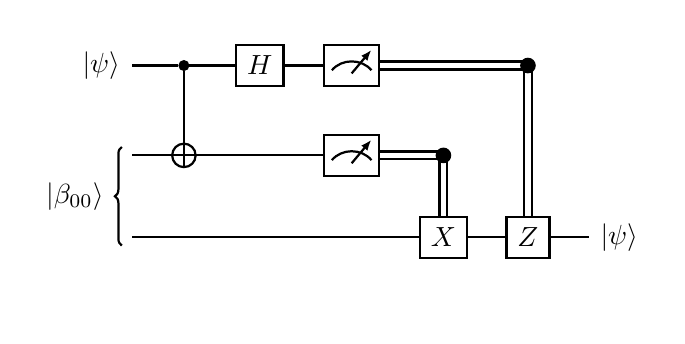
\begin{tikzpicture}
        \node[scale=1.0] {
            \begin{quantikz}
                \lstick{$\ket{\psi}$}                & \ctrl{1} & \gate{H} & \meter{} & \cw        & \cwbend{2} \\
                \lstick[wires=2]{$\ket{\beta_{00}}$} & \targ{}  & \qw      & \meter{} & \cwbend{1} \\
						       \qw      & \qw      & \qw      & \qw        & \gate{X}   & \gate{Z} & \qw \rstick{$\ket{\psi}$}\\
            \end{quantikz}
        };
    \end{tikzpicture}
    \caption{Quantum teleportation circuit}
    \label{fig:teleport}
\end{figure}

\lstinputlisting[language=QHaskell,lastline=10,caption=Quantum teleportation]{teleport.qh}

\clearpage

Verification steps follow:

\lstinputlisting[language=QHaskell,firstline=12,caption=Annotated quantum teleportation program]{teleport.qh}

At line 16, something interesting happens! When we measure a quantum variable (in the default computational basis), its state is collapsed to either 0 or 1 based on the distribution of either outcomes. In our logic, however, both the outcome and the distribution are still maintained. This is achieved by replacing the measured qubit (which is implicitly discarded with the measurement operation) in the subsystem under consideration with a ghost variable. If the quantum variable was previously entangled, it is replaced with a entangled ghost ($e$) and if it was unentangled with an unentangled ghost ($u$). Further, we maintain the correspondence between the classical bit that stores the measurement result and the ghost variable that replaced its corresponding qubit. So above, $e_x$ corresponds to the classical bit $x$. Similarly, in lines 20-22, $e_y$ is introduced corresponding to $y$. This helps us in the following two steps of the program where operations controlled on the previous measurement outcomes are applied. We recover the original state $\ket{\psi}$ at the end.

\subsubsection{Fair coin toss}

Here we write a program along with its verification steps which produces a uniformly random bit:

\lstinputlisting[language=QHaskell,firstline=8,caption=Fair coin toss]{cointoss.qh}

In this program we see the use of an unentangled ghost variable ($u_x$) at line 8 that records the outcome distribution of the measured qubit whose result is stored in the classical bit $x$.

\section{Discussion and related work}

In \cref{sec:teleport}, when we presented code for quantum teleportation, it is not apparent from its type (or specification) whether the quantum variables q (input) and b (output) are different. We can improve the specification by requiring the Bell state, $\ket{\beta_{00}}$, to be part of the input, but this requires changing the implementation as well. Another solution could be to specify that q is discarded in the postcondition (equivalent to saying that it gets consumed). This latter solution, although not currently expressible in our system, could be better. Even better would be to have a way to specify information about the resource usage of the program; in teleportation, for example, an EPR pair gets consumed along with the input qubit.

\section{Conclusion and perspectives}

\blindtext

\section*{Acknowledgements}
\blindtext

\bibliographystyle{eptcsalpha}
\bibliography{references}

\clearpage

\appendix

\section{Metatheory}

\blindtext

\end{document}
